% !TeX program = xelatex
% 使用 XeLaTeX 或 LuaLaTeX 编译。Overleaf 请在 Menu -> Compiler 选择 XeLaTeX。
\documentclass{BJUTReport}

\usepackage{graphicx}
\usepackage{booktabs}
\usepackage{float}
\usepackage{amsmath}
\graphicspath{{Fig/}{../outputs/figures/}}

%%%%%%%%%%%%%%% 报告题目
\newcommand{\thesisTitle}{大语言模型空间建模能力的认知边界与逻辑一致性挖掘分析}

%%%%%%%%%%%%%% 个人信息：提交前按实际情况修改
\newcommand{\yourDept}{信息学部（请按实际学院修改）}
\newcommand{\yourMajor}{计算机类 / 数据科学与大数据技术（请按实际专业修改）}
\newcommand{\yourName}{张驰}
\newcommand{\yourMentor}{（请填写指导教师）}
\newcommand{\yourjob}{（请填写职称）}
\newcommand{\studentID}{23070215}
\newcommand{\yourYear}{2026}
\newcommand{\yourMonth}{5}
\newcommand{\yourDay}{6}

% ==================== 原创声明信息 ====================
\signauthor{张驰}
\signsupervisor{（请填写指导教师）}
\signyear{2026}
\signmonth{5}
\signday{6}

\begin{document}

\coverpage

\begin{authorization}
\end{authorization}

\begin{abstract}
本文围绕“电动轮椅能否在狭窄楼梯转角处完成 90 度转弯”这一空间推理任务，构建多层级 Prompt 数据集，将大语言模型的回答视为可挖掘的行为数据，分析模型在自然语言描述、参数化描述和数学建模描述之间的判断稳定性与认知边界。实验设计包括 20 个空间场景、3 个描述层级和 5 类无关干扰条件，形成 300 条基础 Prompt；随后采集模型回复，并抽取最终判断、推理步骤、公式使用、坐标系使用和错误类型等行为特征。分析阶段采用准确率统计、噪声翻转率、层级一致性、决策树、K-Means 聚类和 FP-Growth 关联规则等方法，识别模型在空间建模任务中的典型失效模式。本文当前为报告框架版本，后续可在真实模型采集完成后补充具体数值、图表解释和结论。
\keywords{大语言模型；空间推理；数据挖掘；Prompt 工程；关联规则；聚类分析}
\end{abstract}

\begin{abstractEN}
{Mining Cognitive Boundaries and Logical Consistency of Large Language Models in Spatial Reasoning}
{Zhang Chi}
{Faculty of Information Technology}
{This report studies the cognitive boundaries of large language models in a spatial reasoning task. Taking the wheelchair turning problem in a narrow stair corner as the fixed scenario, the project constructs prompts with different description levels and irrelevant perturbations, collects model responses, and extracts behavioral features such as final judgment, reasoning steps, formula usage, coordinate-system usage, and error category. The analysis framework combines descriptive statistics, noise-induced flip rate, level consistency, decision tree analysis, K-Means clustering, and FP-Growth association rule mining. This version provides a structured report framework for the current project and can be extended with final experimental numbers after data collection is completed.}
\keywordsEN{Large language model; spatial reasoning; data mining; prompt engineering; association rule mining; clustering}
\end{abstractEN}

\contentpage

\section{绪论}

\subsection{研究背景}

大语言模型在常识问答、代码生成和文本分析等任务中表现突出，但其是否真正具备稳定的空间建模能力仍需要通过可控实验验证。空间推理问题通常同时包含自然语言理解、几何约束识别、数量关系比较和逻辑一致性保持等要求，因此适合作为分析模型认知边界的实验载体。

本项目选择“电动轮椅在狭窄楼梯转角处能否顺利完成 90 度转弯”作为固定任务。该问题具有现实空间约束，同时又可以被改写为自然语言描述、参数化描述和形式化建模描述三种层级。与直接求解几何可通行性不同，本报告关注的是模型如何回答、为何出错，以及哪些描述变化会诱发回答翻转。

\subsection{研究目标}

本报告拟完成以下目标：

\begin{itemize}
    \item 构建包含描述层级、干扰条件和场景临界性的 Prompt 实验矩阵；
    \item 自动化采集不同模型在同一空间任务上的回复；
    \item 从回复文本中抽取可量化行为特征；
    \item 使用数据挖掘方法识别模型的准确率差异、逻辑一致性、噪声敏感性和典型失效模式；
    \item 为后续课程报告或论文撰写提供可复现的数据、图表和结论框架。
\end{itemize}

\subsection{本文结构}

第 2 节介绍数据集构造与变量设计；第 3 节说明数据采集与特征工程流程；第 4 节给出数据挖掘方法；第 5 节预留实验结果与分析框架；第 6 节总结当前工作并提出后续完善方向。

\section{数据集构造与实验设计}

\subsection{空间场景生成}

实验以楼梯转角和电动轮椅几何参数为核心，生成多个空间场景。每个场景包含楼梯净宽、平台进深、轮椅宽度、轮椅长度、最小转弯半径等字段。项目中使用的参考余量定义为：

\begin{equation}
margin = \min(W - w,\ D - R)
\label{eq:margin}
\end{equation}

其中，$W$ 表示楼梯通道净宽，$w$ 表示轮椅宽度，$D$ 表示平台有效进深，$R$ 表示保守转弯半径。该参考余量不直接告诉模型，而是用于实验标注与后续评价。

\subsection{Prompt 描述层级}

实验将同一空间场景转写为三个描述层级，如表 \ref{tab:levels} 所示。

\begin{table}[H]
  \centering
  \caption{Prompt 描述层级设计}
  \begin{tabular}{lll}
    \toprule
    \textbf{层级} & \textbf{描述方式} & \textbf{目的} \\
    \midrule
    L1 & 自然语言描述 & 测试模型是否依赖空间常识和直觉判断 \\
    L2 & 具体参数描述 & 测试模型能否正确使用尺寸和阈值信息 \\
    L3 & 数学建模描述 & 测试模型面对形式化几何约束时的稳定性 \\
    \bottomrule
  \end{tabular}
  \label{tab:levels}
\end{table}

\subsection{干扰条件设计}

为了检验模型是否会被无关环境信息带偏，实验为每个 Prompt 设置 5 类干扰条件：无干扰、材质颜色、环境噪声、光照条件和情绪压力。干扰项本身不改变空间几何约束，但可能影响模型的语义注意力分配。

\begin{table}[H]
  \centering
  \caption{无关干扰条件}
  \begin{tabular}{ll}
    \toprule
    \textbf{干扰标签} & \textbf{示例内容} \\
    \midrule
    none & 不添加无关信息 \\
    material\_color & 楼梯扶手颜色、墙面材质 \\
    ambient\_noise & 现场说话声和环境噪声 \\
    lighting & 光照偏暗、地面干燥等状态 \\
    emotional\_pressure & 使用者着急、旁观者催促 \\
    \bottomrule
  \end{tabular}
  \label{tab:noise}
\end{table}

\subsection{数据规模}

默认配置包含 20 个空间场景、3 个描述层级和 5 类干扰条件，因此单模型单轮采样形成：

\begin{equation}
20 \times 3 \times 5 = 300
\label{eq:prompt-size}
\end{equation}

条 Prompt。若比较 3 个模型并重复采样 3 次，则总回复量可达到 $300 \times 3 \times 3 = 2700$ 条。

\section{数据采集与特征工程}

\subsection{采集流程}

项目通过 Python 脚本完成从 Prompt 生成到模型回复采集的流程。核心文件包括：

\begin{itemize}
    \item \verb|scripts/01_generate_prompts.py|：生成 Prompt 矩阵；
    \item \verb|scripts/02_collect_responses.py|：调用 mock 或真实模型 API；
    \item \verb|scripts/03_build_features.py|：从回复文本中抽取行为特征；
    \item \verb|scripts/04_analyze.py|：执行统计分析、聚类和关联规则挖掘。
\end{itemize}

采集脚本支持断点续采，能够跳过已经存在的 $(model, repeat, prompt\_id)$ 组合，避免 API 调用重复。

\subsection{行为特征抽取}

模型原始回复存储在 \verb|data/raw/model_responses.csv| 中。随后，项目从回复文本中抽取以下行为特征：

\begin{table}[H]
  \centering
  \caption{模型回复行为特征}
  \begin{tabular}{ll}
    \toprule
    \textbf{字段} & \textbf{含义} \\
    \midrule
    ai\_judgment & 模型最终判断，包含能通过、不能通过、不确定 \\
    is\_correct & 模型判断是否与参考标签一致 \\
    reasoning\_steps & 回复中的推理步骤数量 \\
    has\_formula & 是否出现公式、比较符号或变量表达 \\
    uses\_coordinate & 是否使用坐标系、包络线等建模语言 \\
    error\_category & 错误回复对应的失效模式类别 \\
    \bottomrule
  \end{tabular}
  \label{tab:features}
\end{table}

\subsection{失效模式标注}

本项目将错误回复初步归纳为以下几类：概念混淆、计算崩溃、直觉过拟合、噪声牵引、单位混乱和信息不足。后续报告可以结合典型样例，说明每类错误在文本中的具体表现。

\section{数据挖掘方法}

\subsection{描述性统计与准确率分析}

首先按模型、Prompt 层级、干扰条件和场景临界性统计准确率。该部分用于回答“哪个模型在哪类描述上更稳定”这一基础问题，并为后续可视化提供数据。

\subsection{层级一致性分析}

层级一致性用于衡量同一场景从 L1 到 L3 描述变化时，模型判断是否保持一致。如果模型在 L3 形式化描述中反而更容易出错，则说明形式化符号并不必然带来更强空间建模能力。

\subsection{噪声翻转率分析}

噪声翻转率衡量加入无关信息后，模型相对无噪声版本的最终判断是否发生变化。该指标可以识别模型是否过度关注颜色、噪声、光照和情绪压力等非几何因素。

\subsection{决策树与聚类分析}

决策树用于解释哪些特征最能区分正确与错误回复；K-Means 聚类用于根据准确率、公式使用率、坐标系使用率、噪声翻转率等指标划分模型行为类型。例如，某些模型可能表现为“符号逻辑型但计算链不稳定”，另一些模型可能表现为“自然语言直觉型但参数敏感性较低”。

\subsection{FP-Growth 关联规则挖掘}

FP-Growth 用于挖掘“条件组合 $\rightarrow$ 结果模式”的关联关系 \cite{han2000mining}。例如，可以分析如下规则：

\begin{equation}
\{level=L3,\ has\_noise=1\} \Rightarrow error\_category=calculation\_collapse
\label{eq:rule}
\end{equation}

这类规则有助于从大量回复中提炼可解释的失效路径。

\section{实验结果与分析框架}

本节为后续完善报告时的结果承载框架。若真实模型采集已经完成，可直接从 \verb|outputs/tables| 与 \verb|outputs/figures| 中补充统计结果。

\subsection{整体准确率}

建议在此处插入 \verb|outputs/tables/accuracy_by_level.csv| 的关键数值，并结合图 \ref{fig:accuracy} 说明不同模型在 L1、L2、L3 下的准确率差异。

\begin{figure}[H]
  \centering
  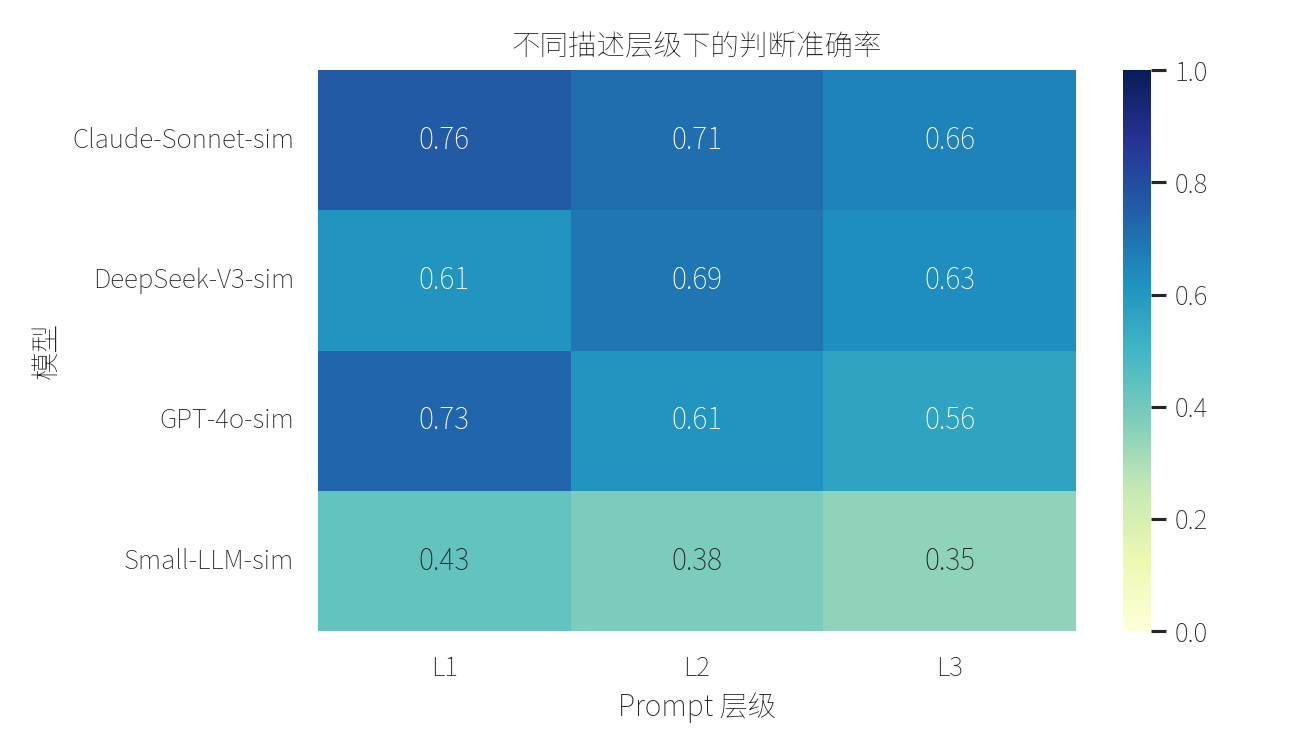
\includegraphics[width=0.82\textwidth]{accuracy_heatmap.png}
  \caption{不同模型在 Prompt 层级上的准确率热力图}
  \label{fig:accuracy}
\end{figure}

\subsection{模型行为边界}

图 \ref{fig:radar} 可用于对比不同模型在准确率、一致性、公式使用、坐标建模和噪声敏感性等维度上的综合表现。正式写作时，应结合具体指标解释各模型的优势和边界。

\begin{figure}[H]
  \centering
  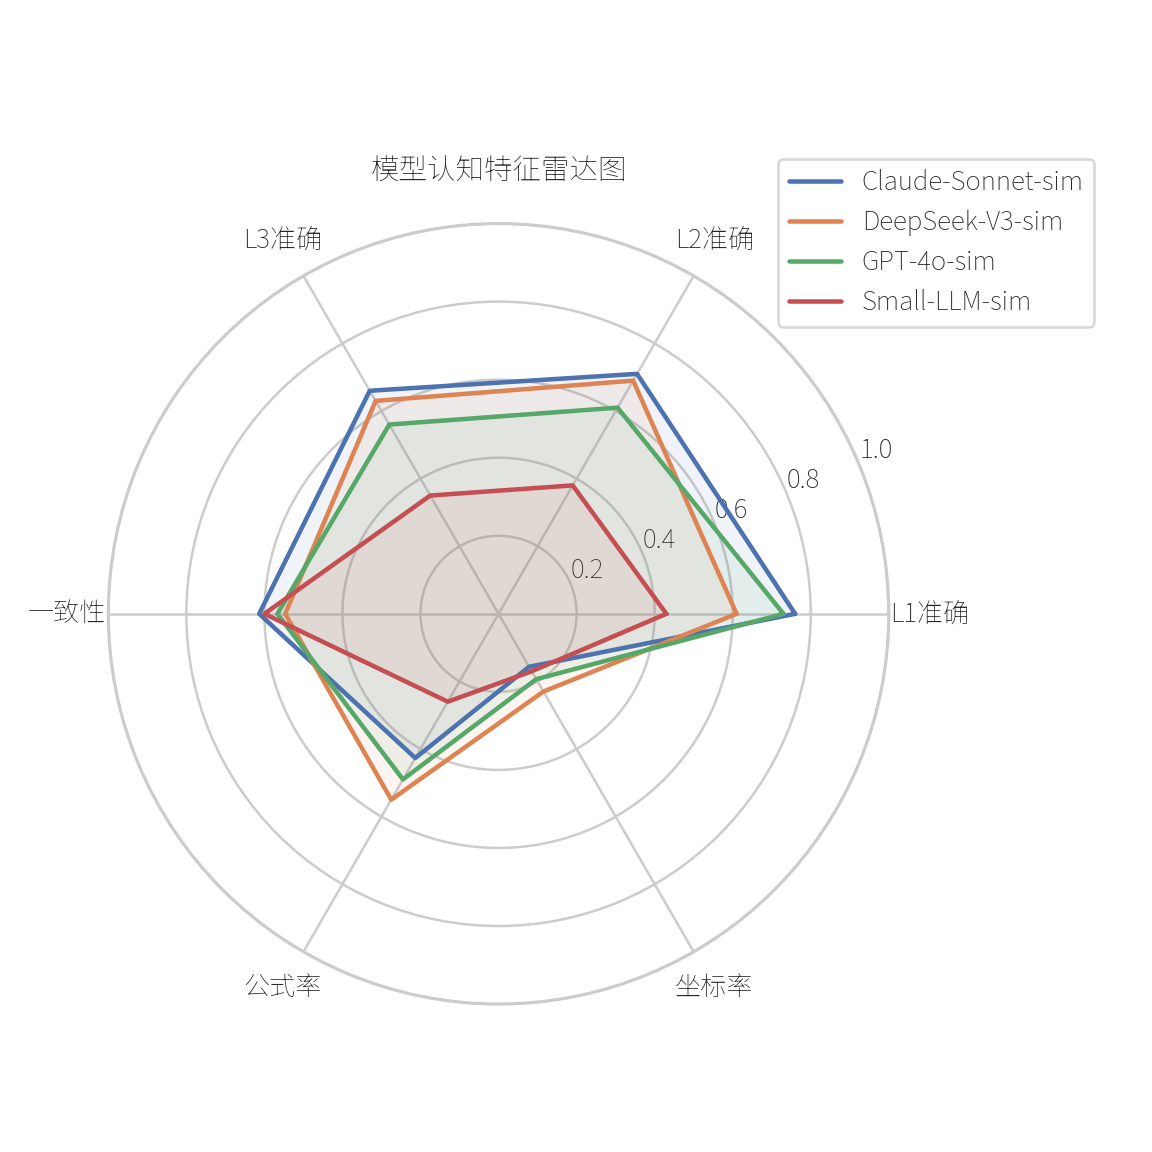
\includegraphics[width=0.78\textwidth]{model_radar.png}
  \caption{模型行为特征雷达图}
  \label{fig:radar}
\end{figure}

\subsection{无关噪声对判断的影响}

该部分可结合 \verb|outputs/tables/noise_flip_rate.csv|，分析不同噪声条件是否引起模型判断翻转。重点关注 borderline 场景，因为临界场景更容易放大模型的不稳定性。

\subsection{失效模式分析}

可结合 \verb|outputs/tables/failure_modes.csv| 和错误样例，分析错误主要集中在哪些类别。建议至少选取 2 到 3 条典型回复，说明模型如何出现概念混淆、计算崩溃或噪声牵引。

\subsection{关联规则发现}

可从 \verb|outputs/tables/outcome_rules.csv| 中选取支持度、置信度和提升度较高的规则，解释“描述层级、干扰条件、临界性”如何共同诱发某类判断或错误模式。该部分是体现数据挖掘方法价值的重点。

\section{总结与展望}

本文构建了一个面向大语言模型空间推理行为的数据挖掘框架。项目通过多层级 Prompt、无关噪声扰动和可解释行为特征，能够从准确率、逻辑一致性、噪声敏感性和失效模式等角度分析模型能力边界。当前版本已经形成完整的代码流程和报告结构，后续可进一步补充真实模型多轮采样结果，并对关键发现进行统计检验。

后续工作可以从三方面展开：第一，扩大模型和重复采样数量，提高结论稳定性；第二，引入更严格的几何基准或人工复核机制，提升参考标签可信度；第三，将该方法扩展到电梯通行、门洞转向、房间路径规划等更多空间任务，以验证模型空间建模能力的泛化边界。

\clearpage\addcontentsline{toc}{section}{参考文献}
\bibliography{references}
\nocite{*}

\appendix
\phantomsection

\section{项目运行命令}

以下命令可用于复现实验流程：

\begin{lstlisting}
python scripts/01_generate_prompts.py
python scripts/02_collect_responses.py --provider mock
python scripts/03_build_features.py
python scripts/04_analyze.py
\end{lstlisting}

若使用真实 API，应先在 shell 中设置环境变量，避免将密钥写入仓库文件。

\section{待补充清单}

正式提交前建议补充以下内容：

\begin{itemize}
    \item 修改封面中的学院、专业、指导教师和职称；
    \item 根据最终采集结果更新摘要中的样本量和结论；
    \item 在第 5 节补充关键表格数值和图表解释；
    \item 从原始回复中挑选典型错误样例；
    \item 检查参考文献是否与正文引用一致。
\end{itemize}

\begin{acknowledgement}

感谢北京工业大学相关课程提供的数据挖掘实践机会。本项目的完成依赖于课程任务对问题定义、数据采集、特征抽取和挖掘分析的完整要求，也受益于开源 Python 生态中 Pandas、scikit-learn、mlxtend、Matplotlib 等工具的支持。后续将继续完善真实模型实验数据和报告中的定量分析部分。

\end{acknowledgement}

\end{document}
